\providecommand{\main}{../../../..}
\documentclass[\main/dresen_thesis.tex]{subfiles}
  \renewcommand{\thisPath}{\main/chapters/monolayers/structureModel/intro}

\begin{document}
  \label{sec:monolayers:structure:semIntro}
  The long-range order of nanoparticle arrays over large areas is quantitatively studied using X-ray and neutron scattering experiments.
  Whereas SEM is a method to obtain a local image of the structure, it leaves the possibility that the actual sample still has great variations across the substrate, which might have been overlooked.
  Also microscopy only gives an idea of the surface of the structure, while to study the vertical structure it becomes necessary to break the sample to image the cross-section locally.
  From grazing-incidence small-angle scattering and reflectometry experiments on the other hand the full average three dimensional information is obtained unbiased and non-destructively from a large area of the sample, which will be discussed extensively in the following.

  Magnetic monolayers from nanoparticles prepared by the acetylacetonate route are discussed and the used models to describe the square array structure are introduced.
  The results of the nuclear structure of the sample will then be a prerequisite to study the magnetic structure of the samples in the following section.
  The extensive study of the vertical structure is performed on monolayers prepared from the previously discussed nanocubes Ac-CoFe-C, which are additionally used in \refch{ch:doublelayers} to discuss double layer structures.
  The lateral structure of monolayers, studied by grazing-incidence small-angle X-ray \& neutron scattering (GISAXS \& GISANS) is discussed for a second batch of nanocubes Ac-CoFe-C-2, which were prepared from acetylacetonates in a similar synthesis procedure.

  \begin{figure}[tb]
    \centering
    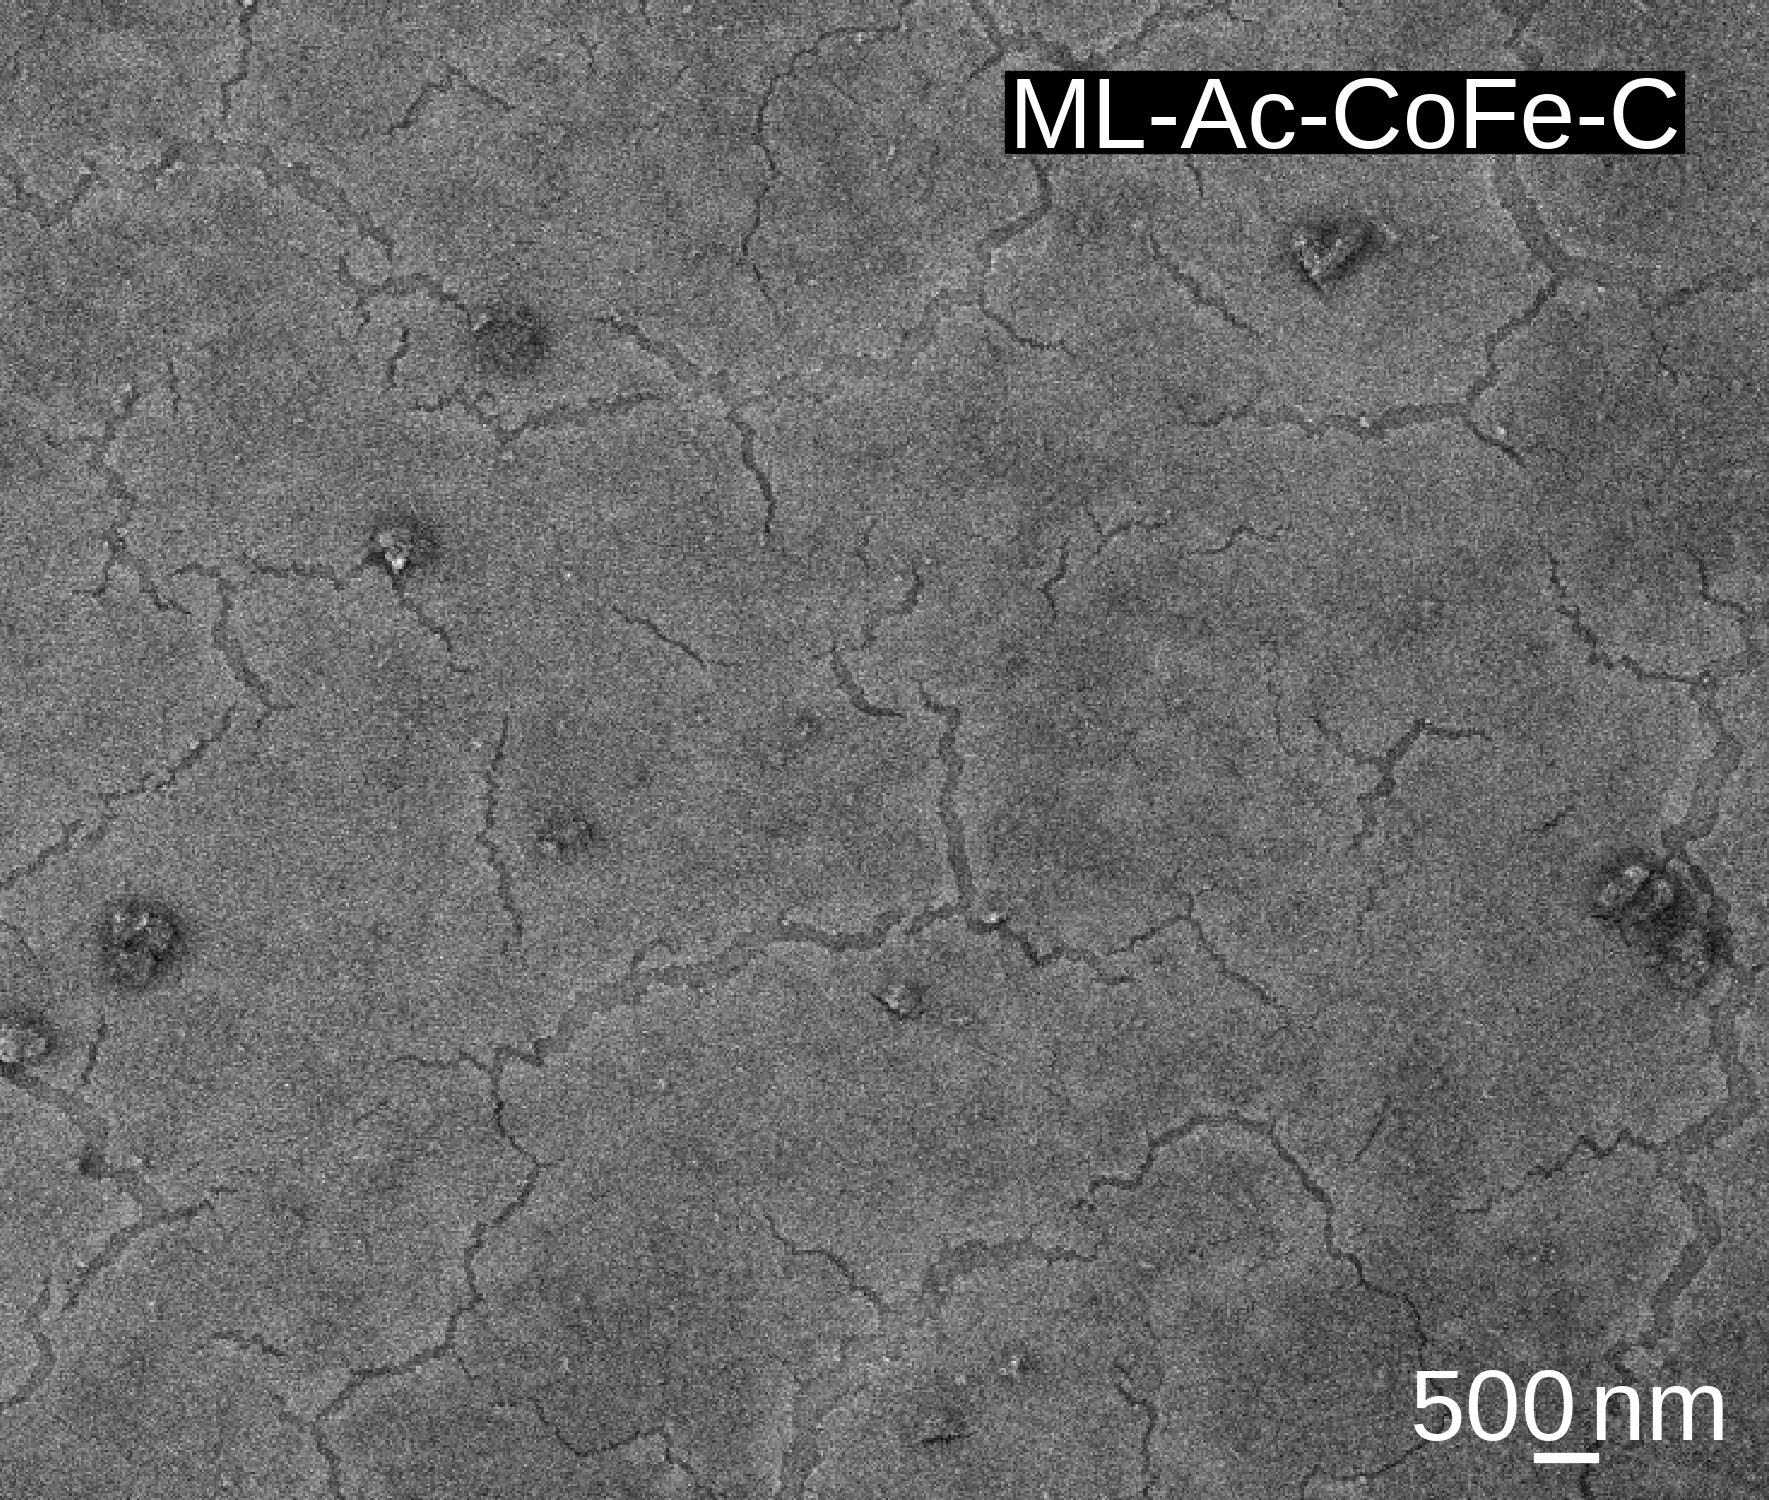
\includegraphics{monolayers_SEM_ML-Ac-CoFe-C_img1}
    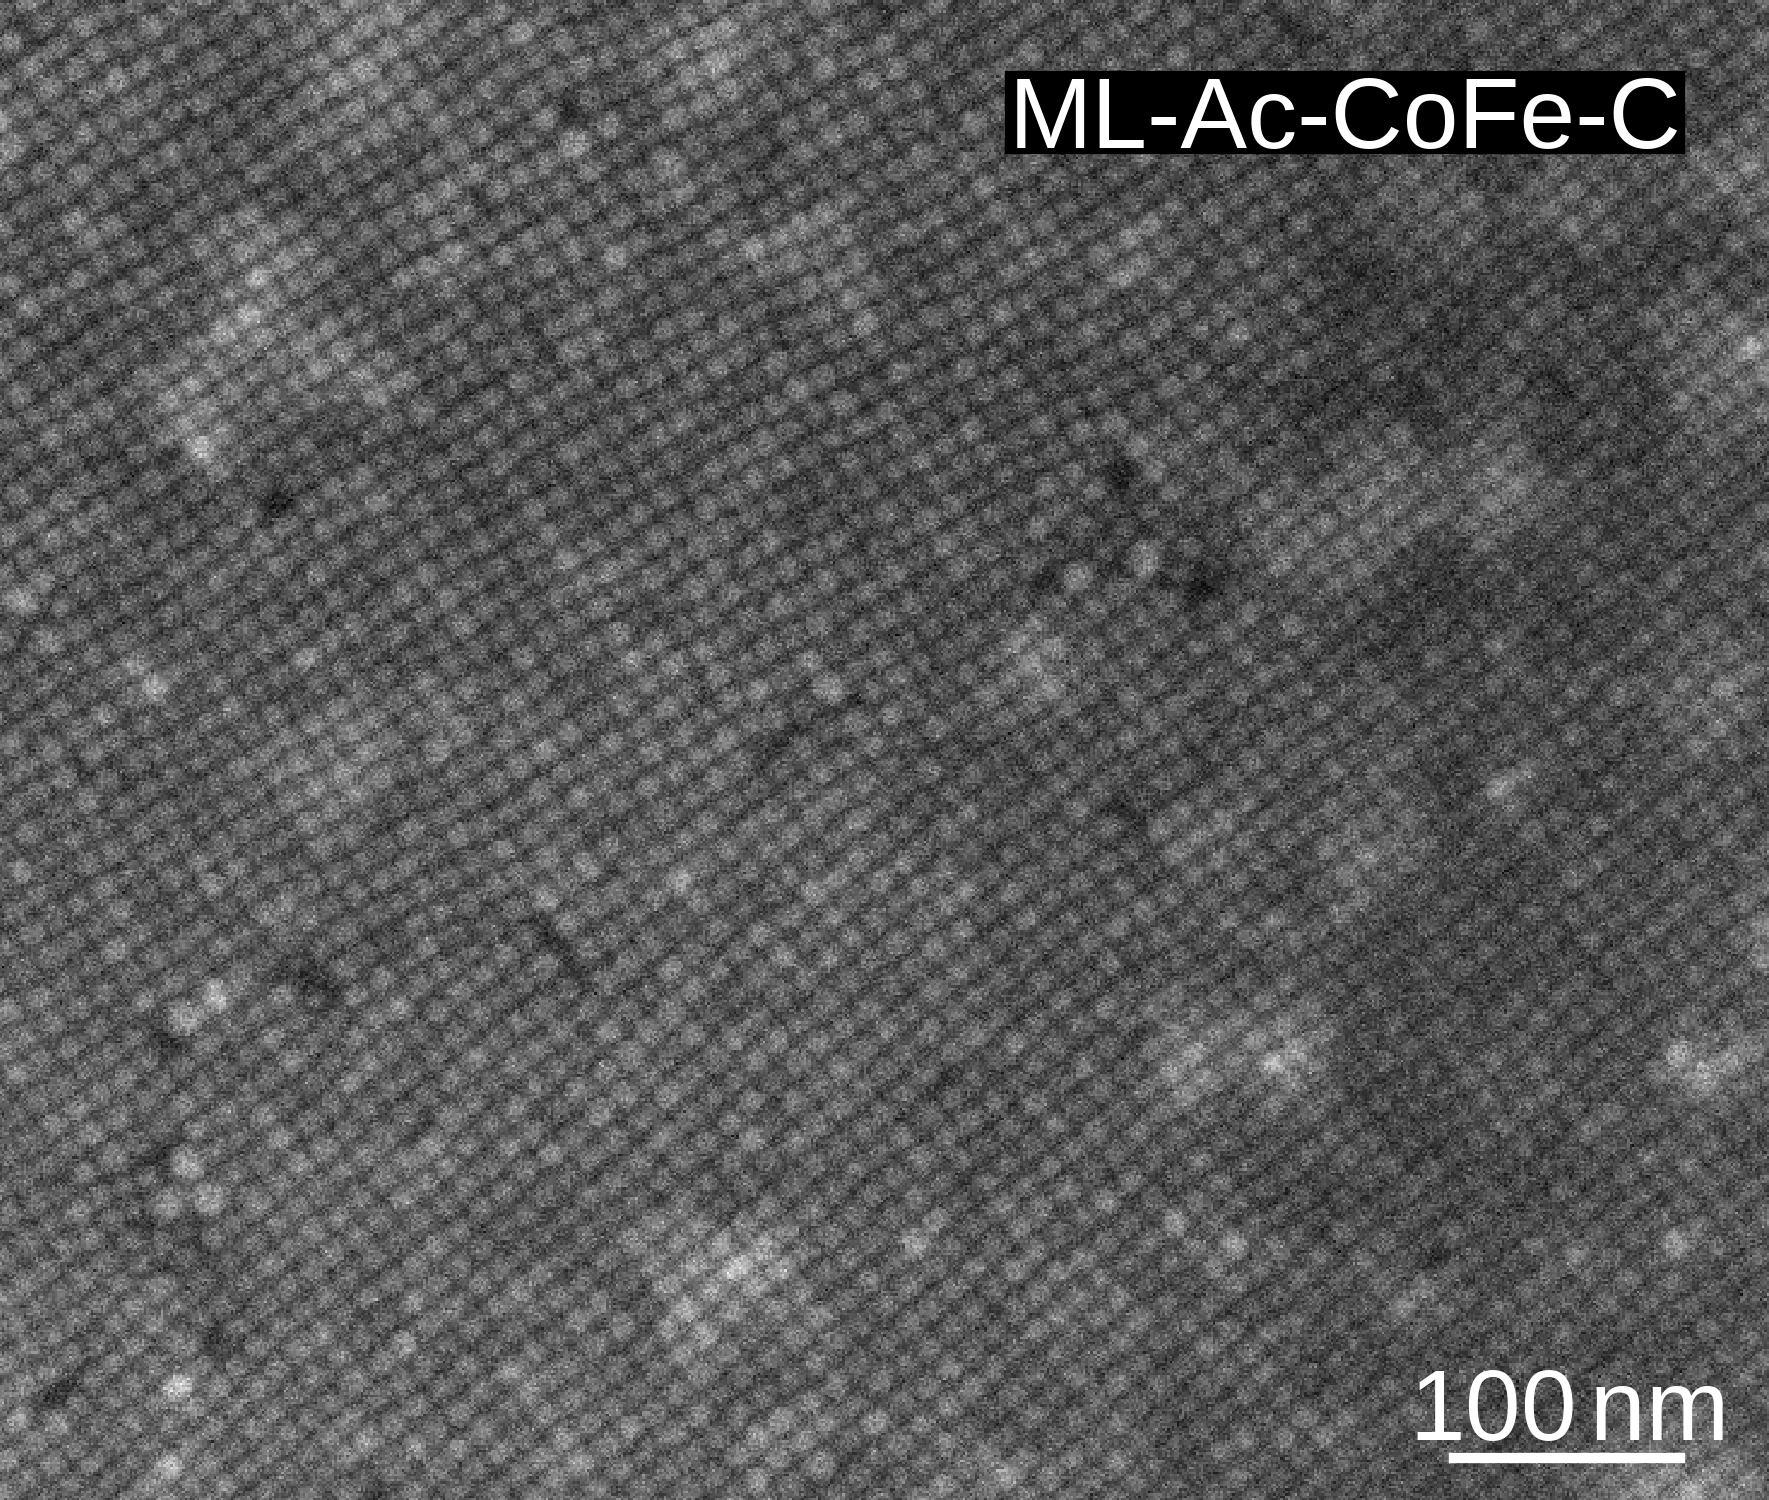
\includegraphics{monolayers_SEM_ML-Ac-CoFe-C_img2}
    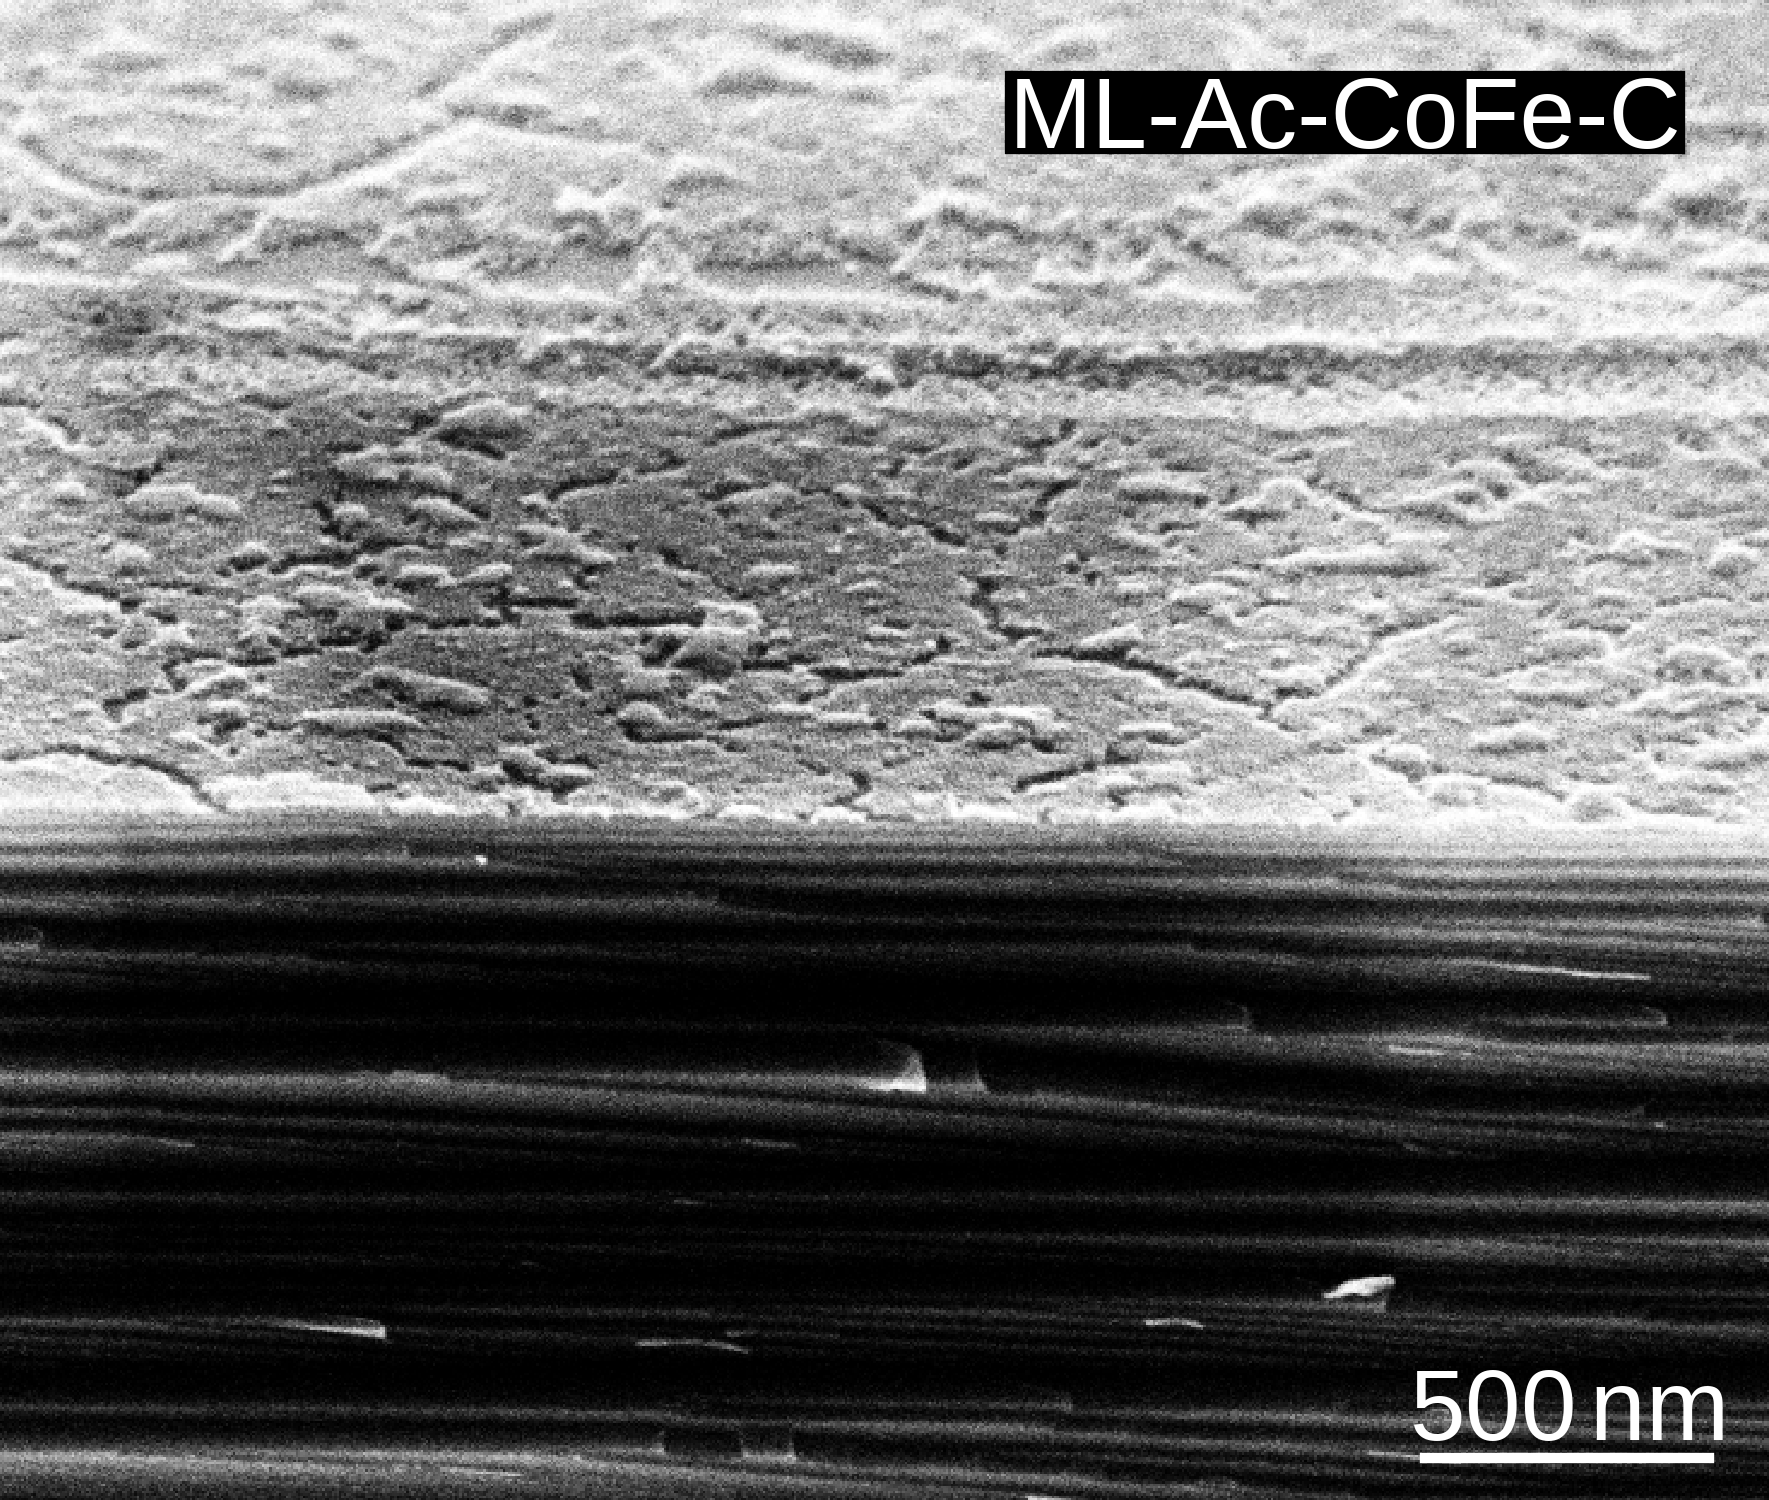
\includegraphics{monolayers_SEM_ML-Ac-CoFe-C_img3}
    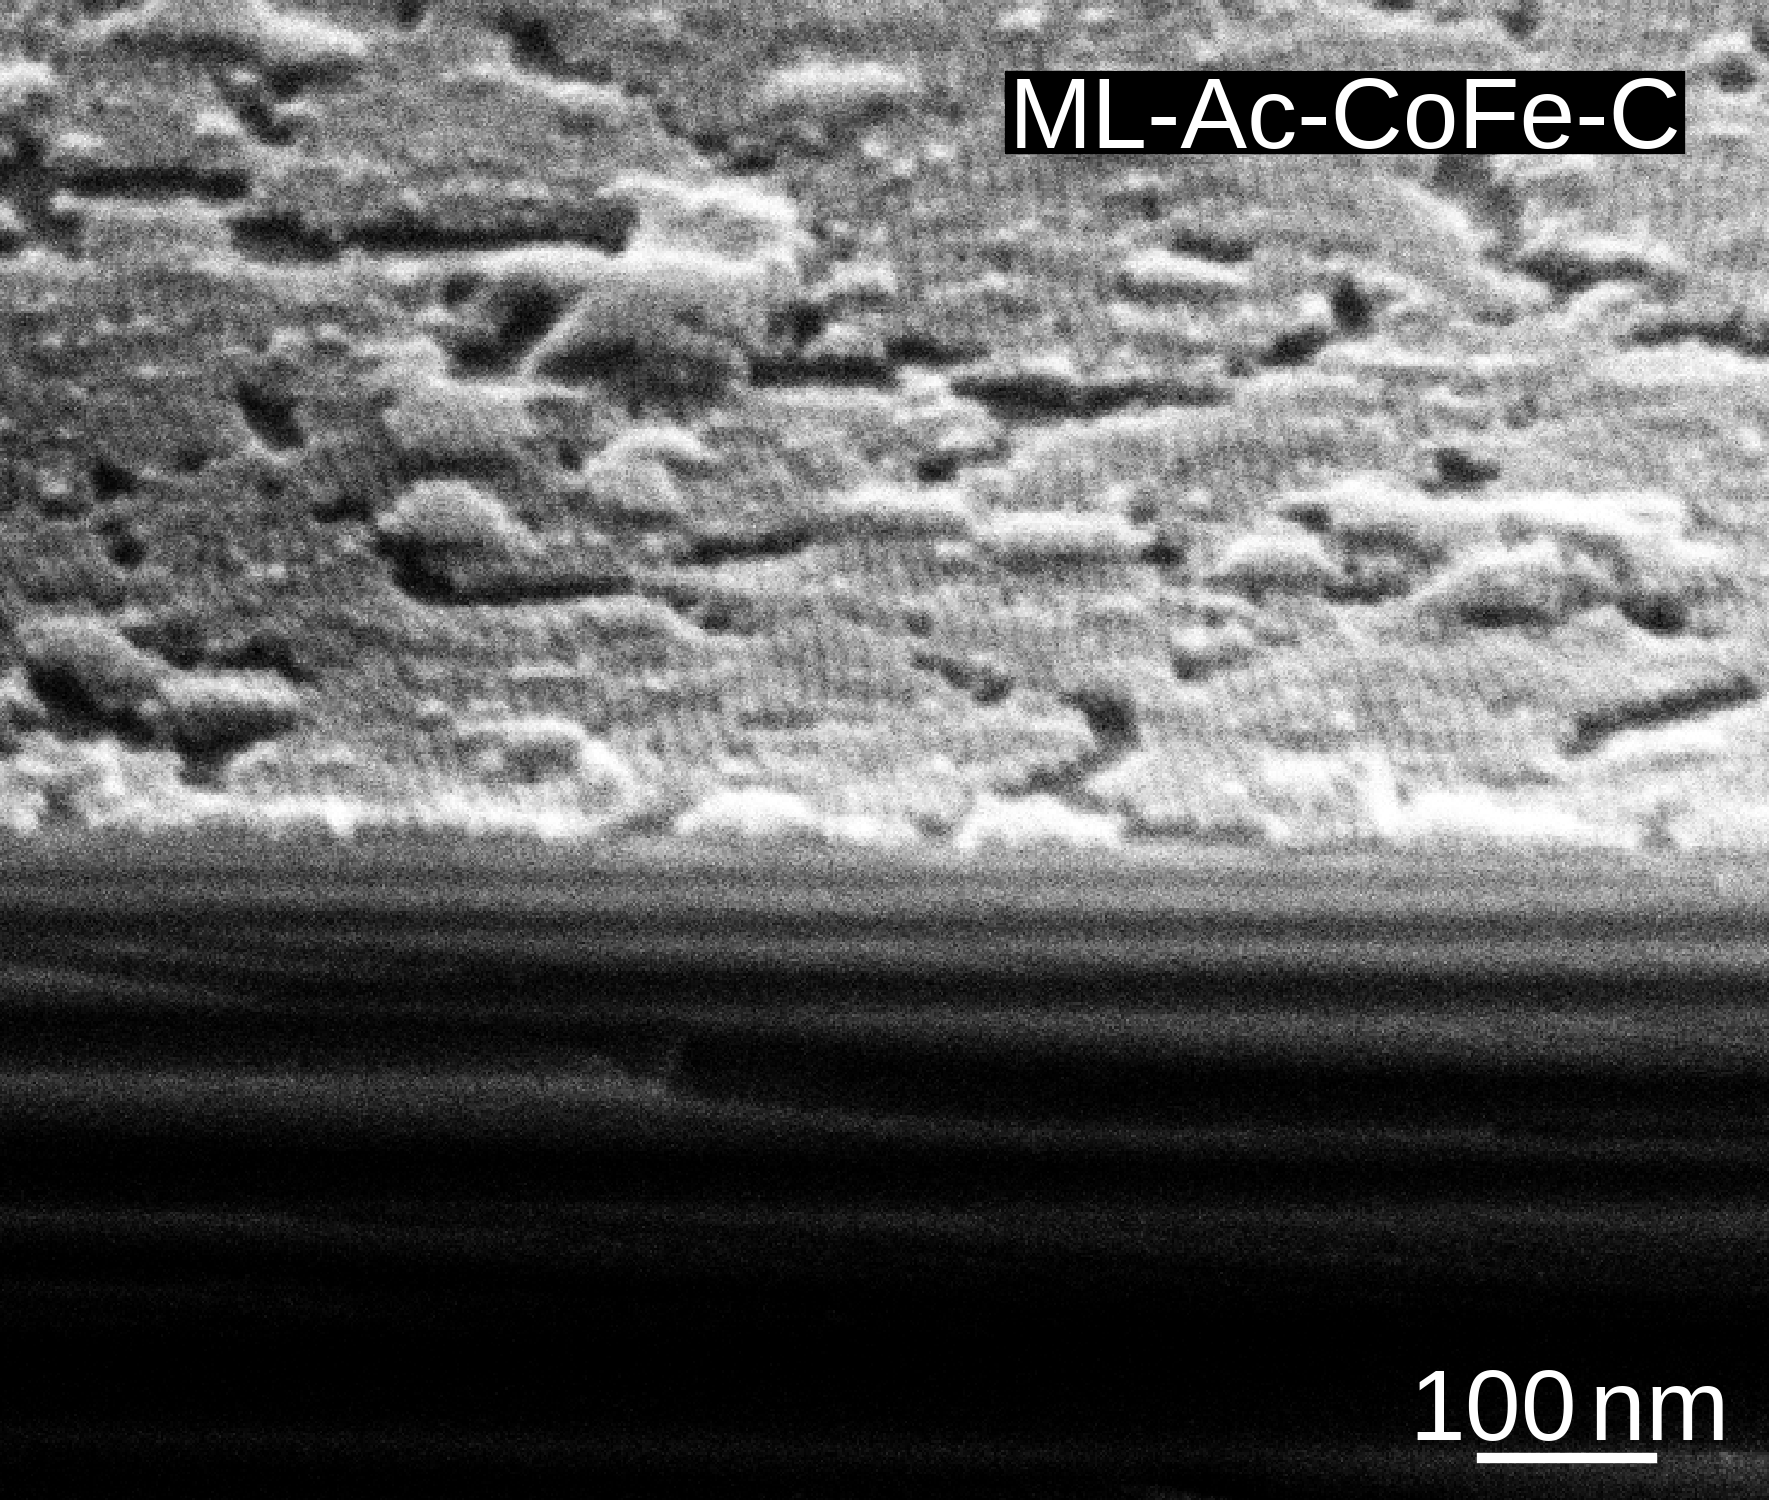
\includegraphics{monolayers_SEM_ML-Ac-CoFe-C_img4}
    \caption{\label{fig:monolayers:structure:semImagesMLACCoFeC}SEM micrographs of a monolayer prepared from Ac-CoFe-C used for the study of the vertical structure of monolayers prepared by the drop casting method.}
  \end{figure}

  \begin{figure}[tb]
    \centering
    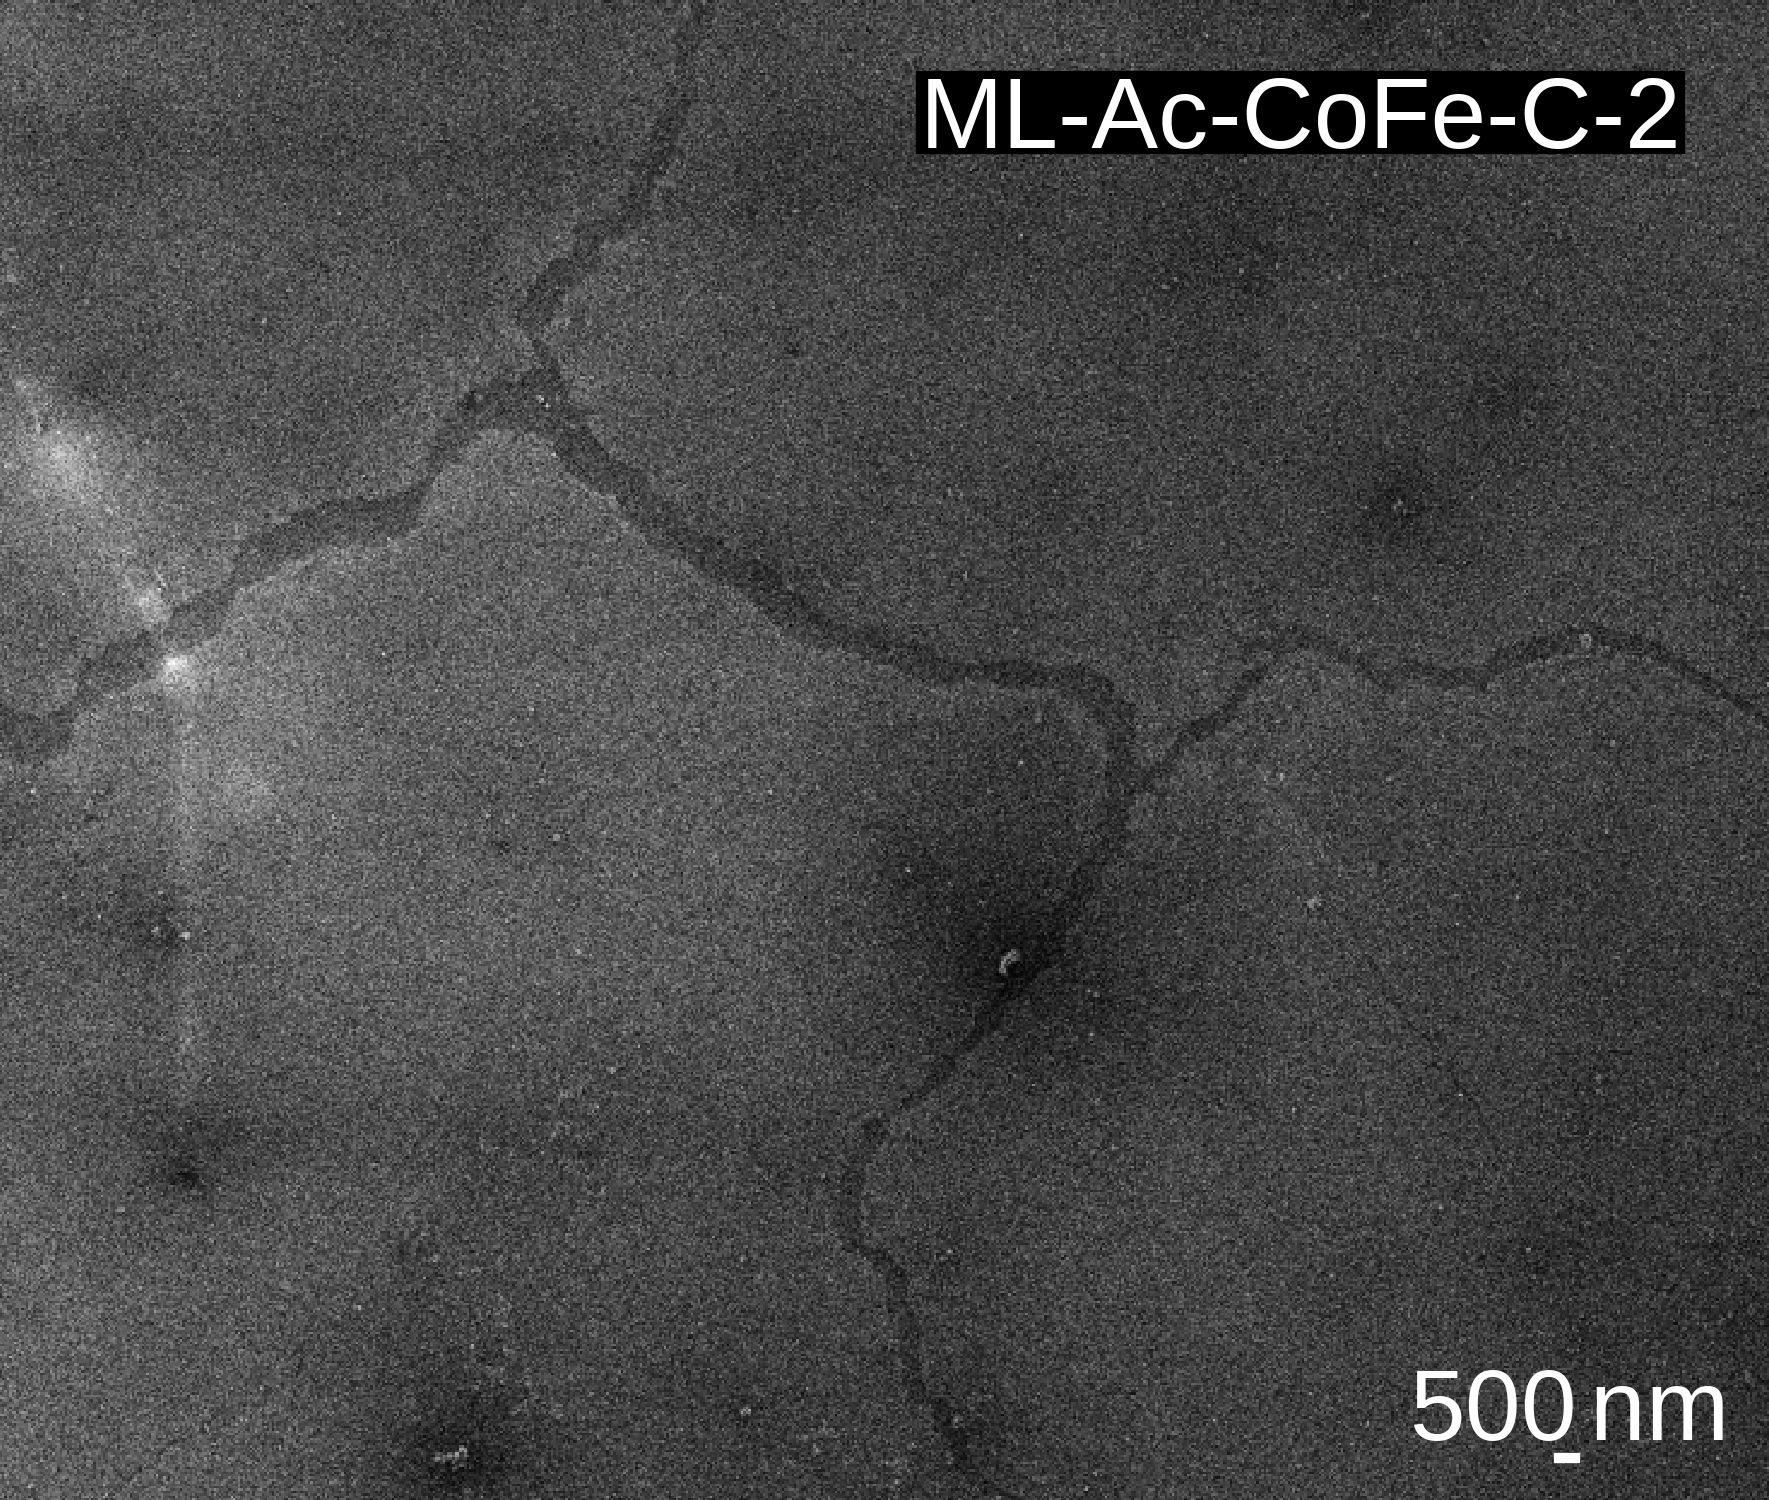
\includegraphics{monolayers_SEM_ML-Ac-CoFe-C-2_img1}
    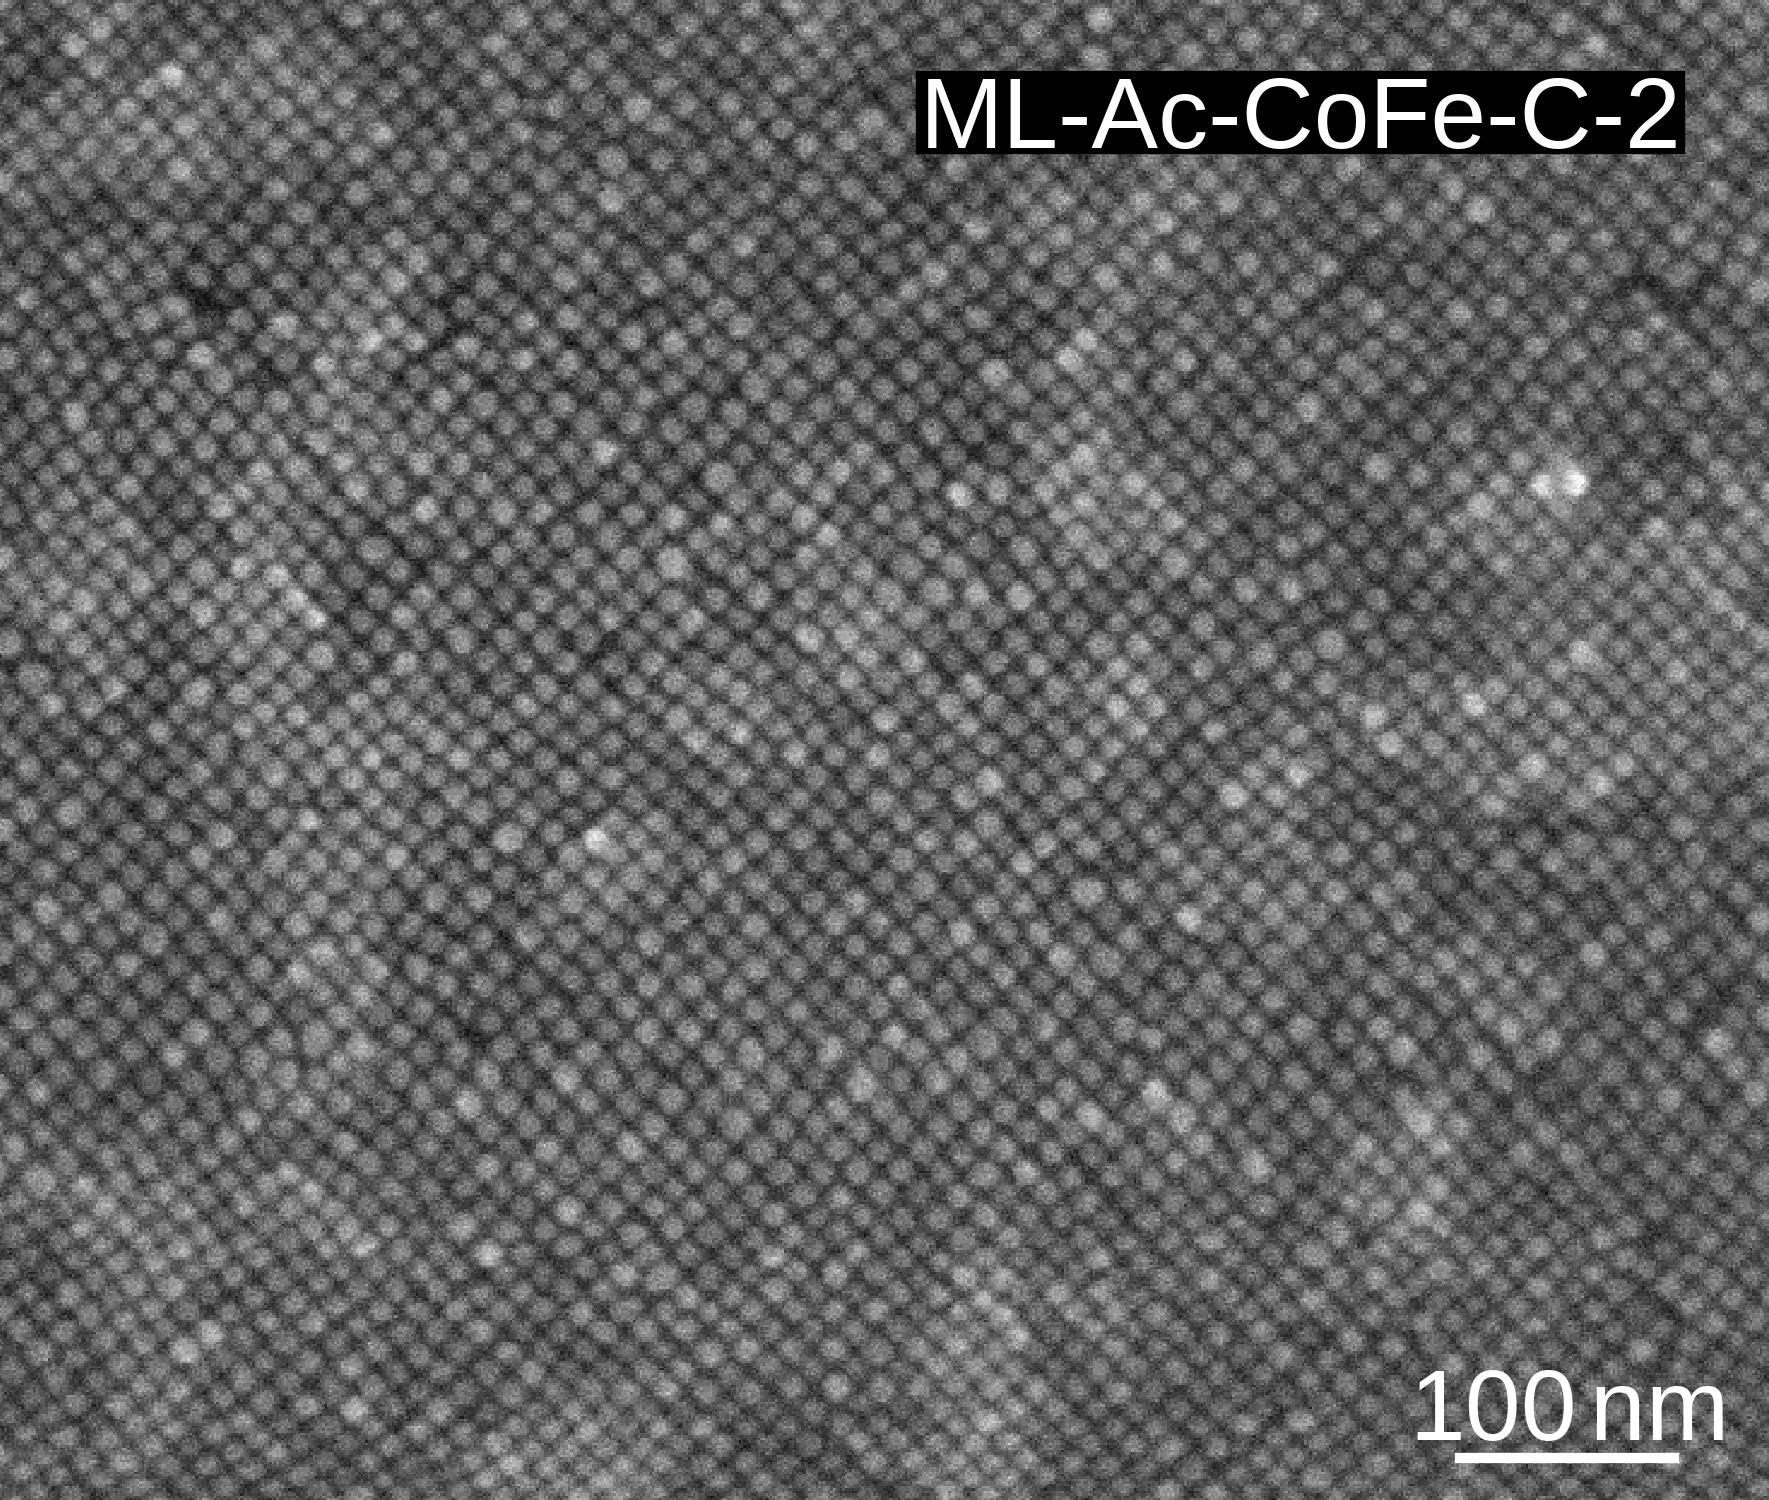
\includegraphics{monolayers_SEM_ML-Ac-CoFe-C-2_img2}
    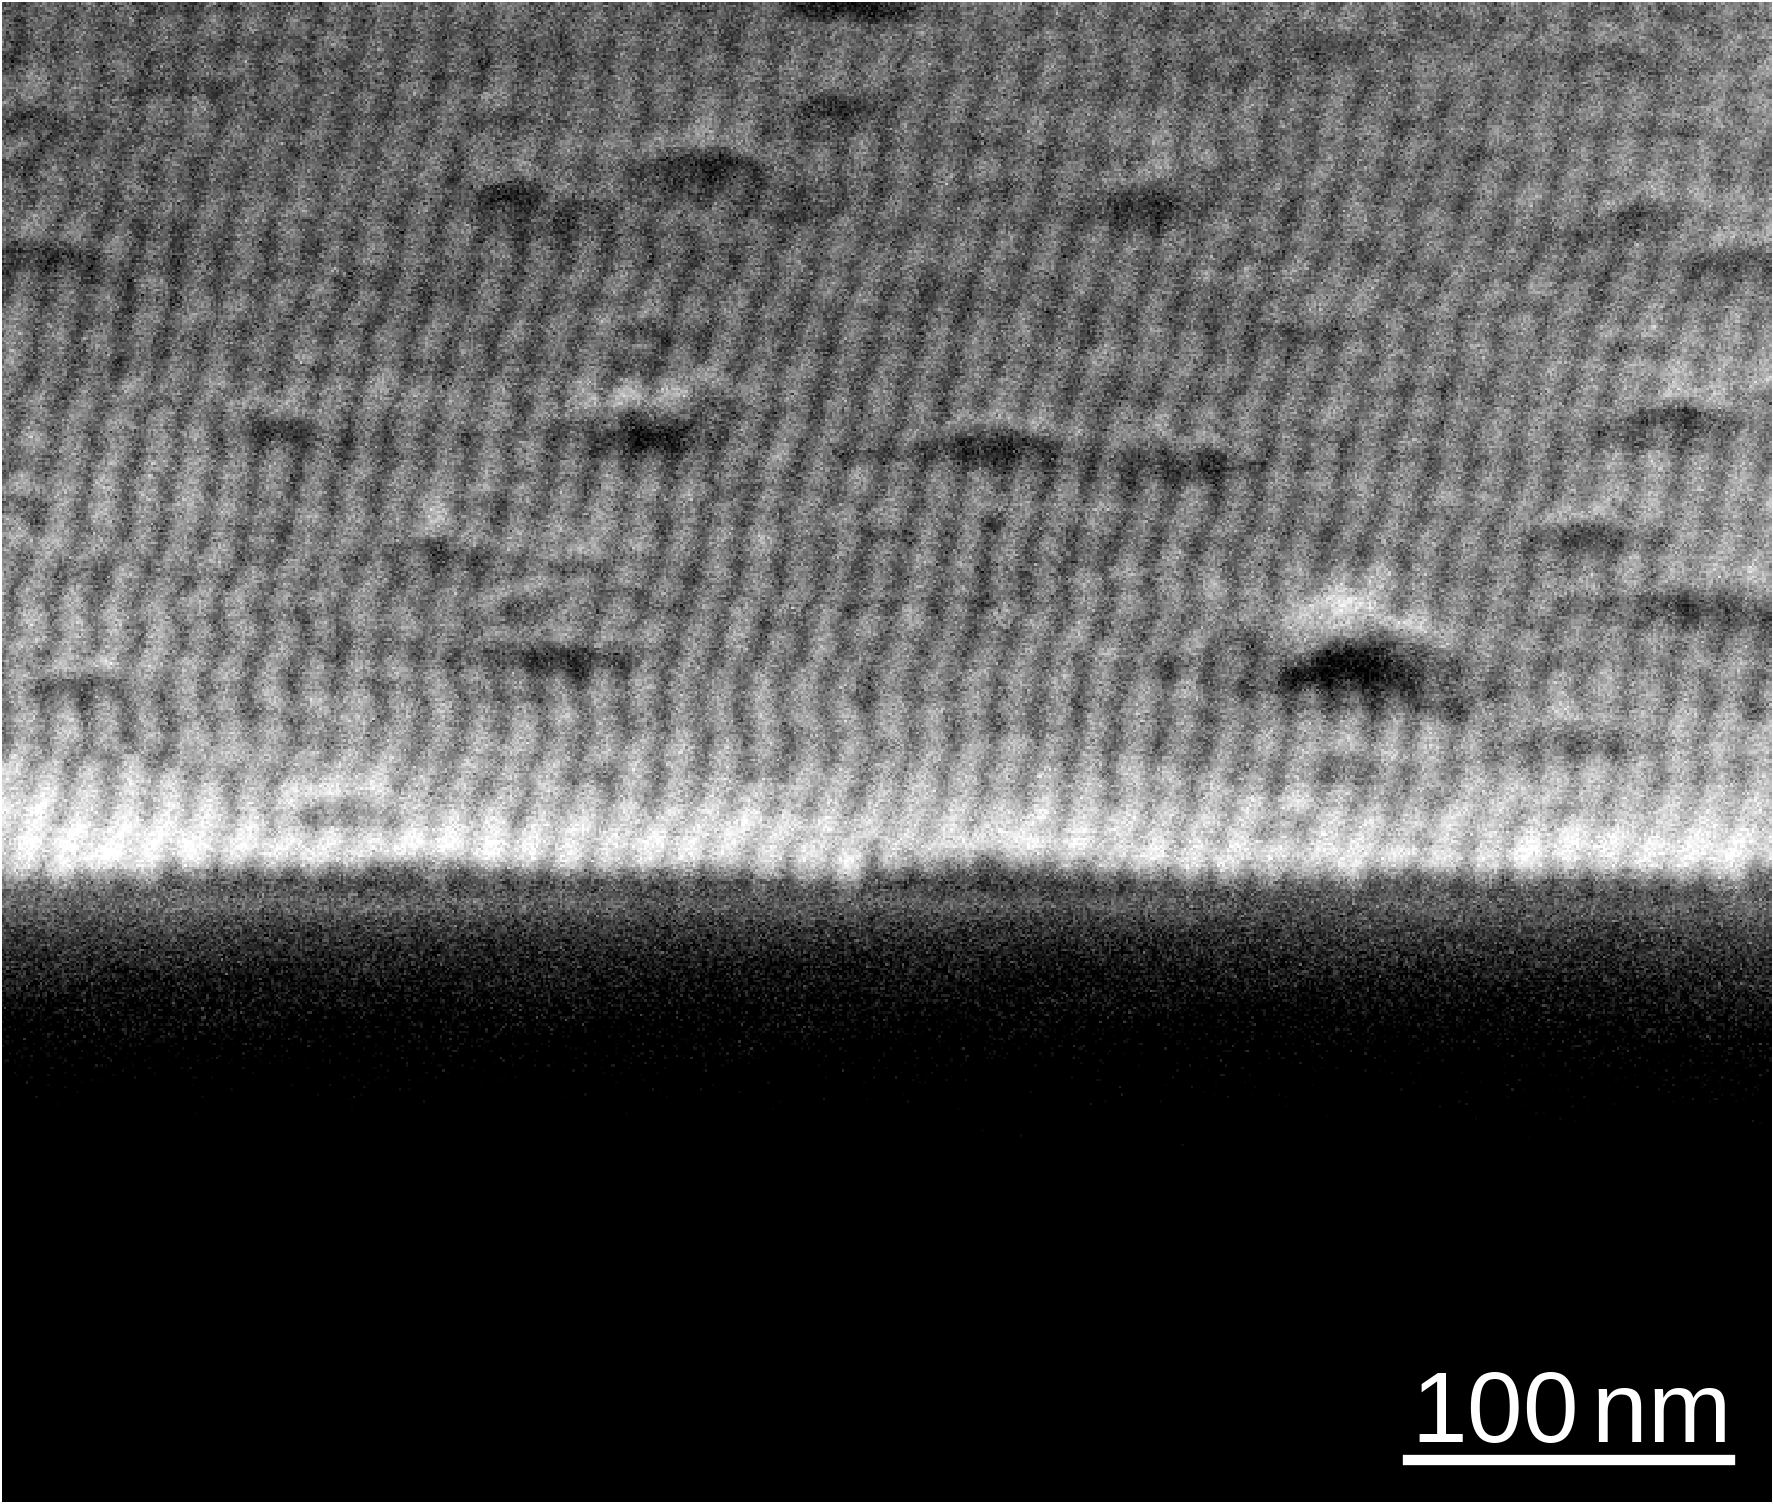
\includegraphics{monolayers_SEM_ML-Ac-CoFe-C-2_img3}
    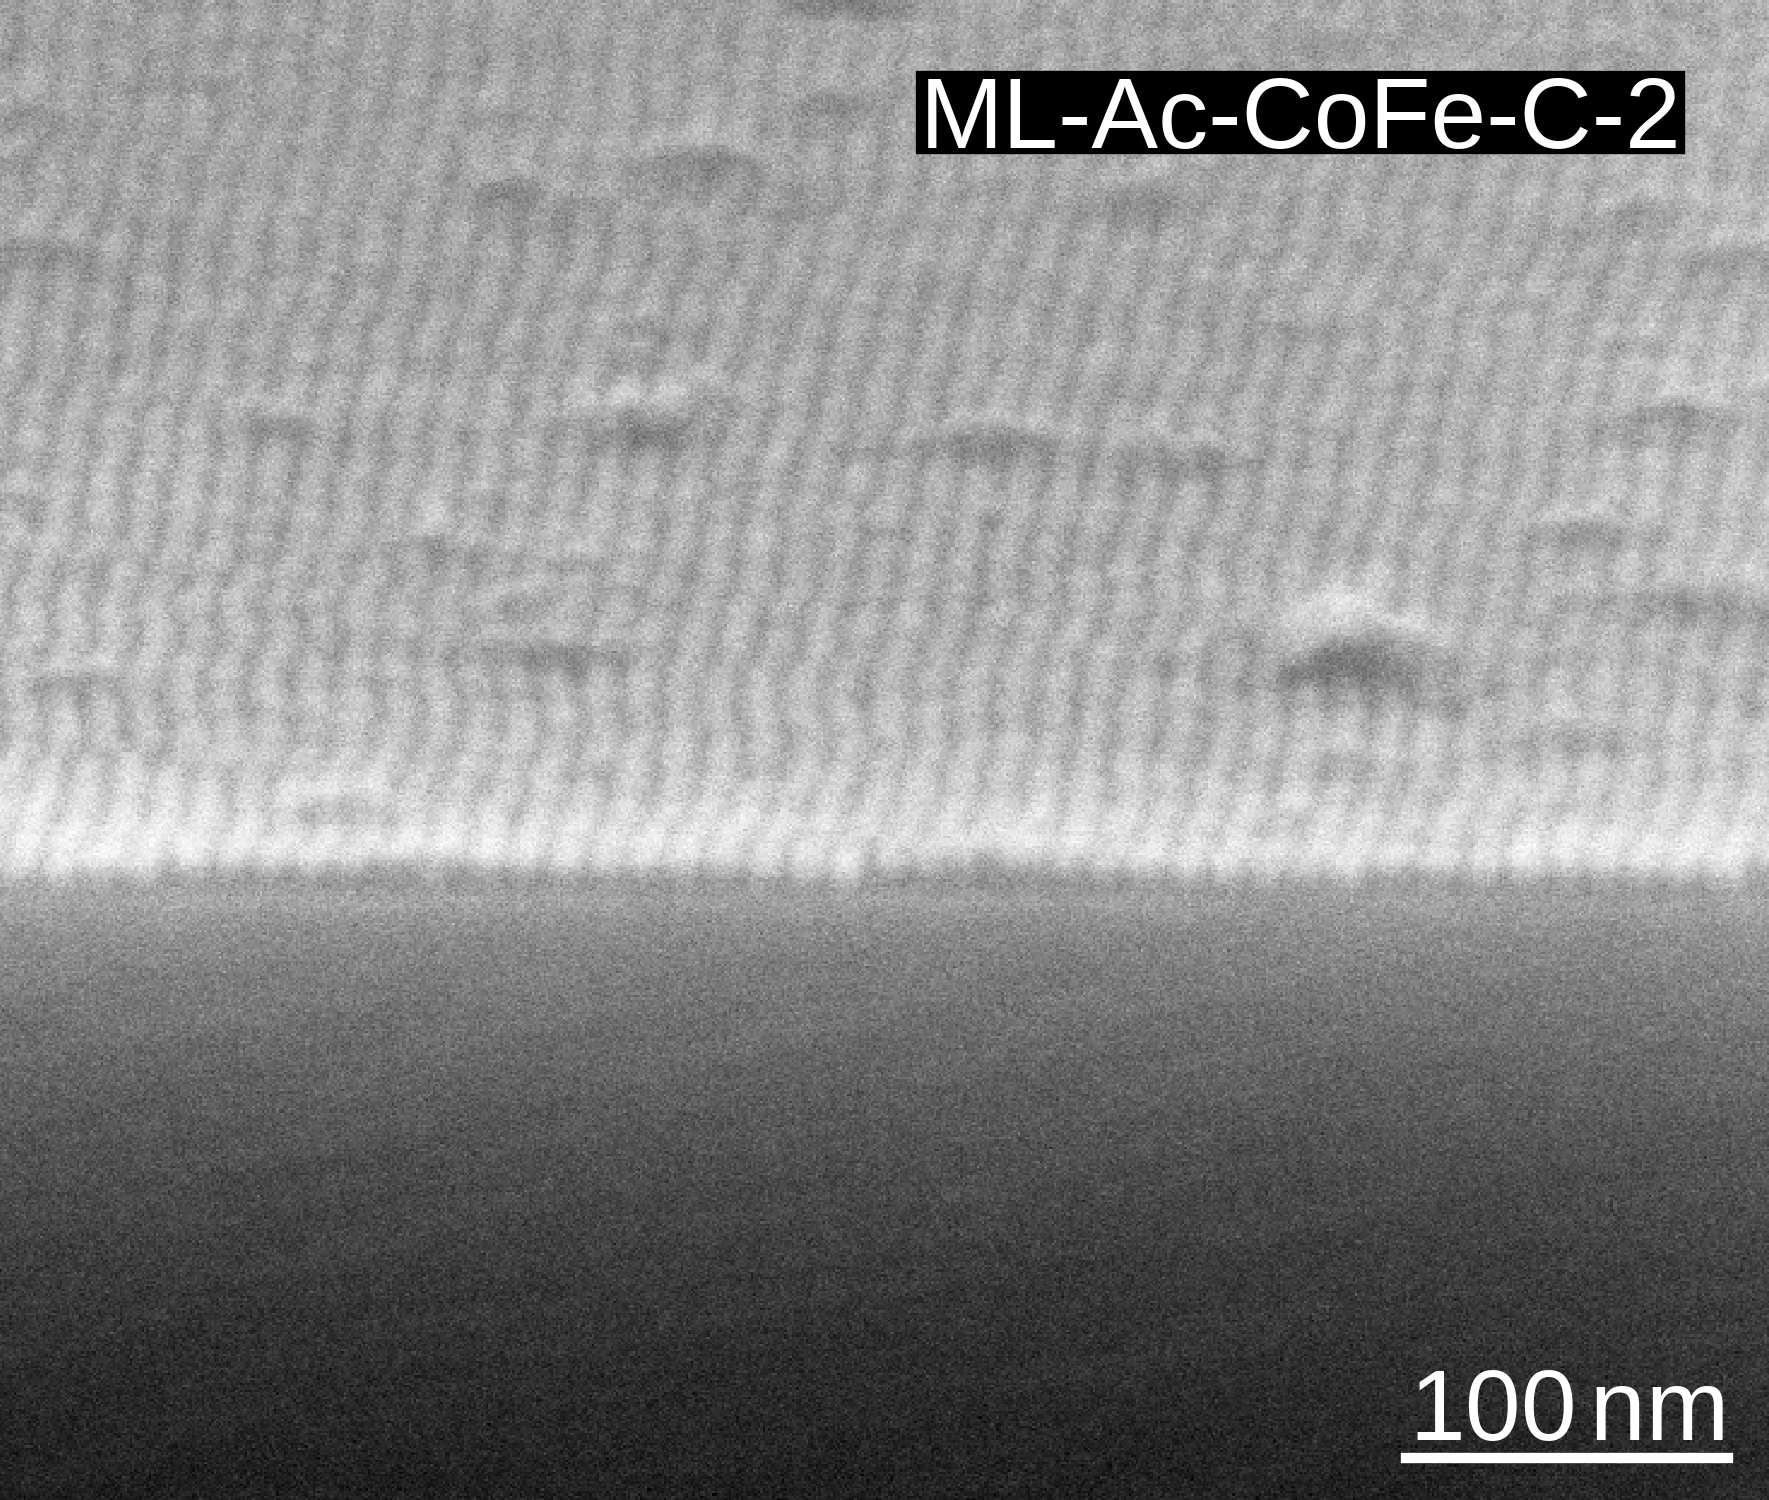
\includegraphics{monolayers_SEM_ML-Ac-CoFe-C-2_img4}
    \caption{\label{fig:monolayers:structure:semImagesMLACCoFeC2}Micrographs of a monolayer ML-Ac-CoFe-C-2 prepared from Ac-CoFe-C-2, which is used for the study of the lateral structure of monolayers by GISAS. The cross-sectional micrographs (lower) are taken from a monolayer that was prepared in parallel to ML-Ac-CoFe-C-2 under the same preparation conditions.}
  \end{figure}

  SEM micrographs for the two studied monolayers ML-Ac-CoFe-C and ML-Ac-CoFe-C-2 are shown in \reffig{fig:monolayers:structure:semImagesMLACCoFeC} and \reffig{fig:monolayers:structure:semImagesMLACCoFeC2}.
  The nanocubes are organized in both cases in a square lattice arrangement and the sample appear to have indeed a single layer structure, as visible from the cross-sectional views.
  It should be noted that the cross-sectional view for ML-Ac-CoFe-C-2 is from a sample that has been prepared in parallel on a second substrate.
  The measurement of a cross-sectional SEM micrograph requires the breaking of the substrate, leaving two smaller sample pieces.
  Neutron scattering experiments, however, require long counting times and therefore a large substrate surface is desired for optimized scattering statistics especially in GISANS experiments, as to why the sample was not broken.

  The square arrays show in both cases cracks on the length scale over a micrometer, whereas ML-Ac-CoFe-C-2 exhibits extended domains in a length scale of $10 \unitmu$.
  The observed cracks appear for multiple reasons.
  According to Bigioni \etal \cite{Bigioni_2006_Kinet}, islands of ordered nanoparticles appear on multiple spots of the droplet surface during the self-assembly process, which then grow to ever larger coherent domains.
  As there is no orientating force, these islands will at some point collide and possibly don't have the freedom anymore to align to one another resulting in the visible cracks in between two orientations.
  Another reason is the relatively large size distribution of both nanoparticle batches.
  The self-assembly process is size-selective in that it favors the alignment of equal sized particles \cite{Rabideau_2007_Obser}.
  Inspecting the cracks shows that in some cases they are filled with particles that are substantially smaller than the average particle size.
  Also it also has to be noted that in both samples, no additional oleic acid had been added to the dispersion before drop casting.\footnote{The reason is that the effect of oleic acid addition was discovered after most X-ray and neutron experiments had been performed.}
  % At last, it should be noted that Ac-CoFe-C-2 shows a stronger magnetism than Ac-CoFe-C, which from the experiment of drop casting within a magnetic field is promoting a better order in the self-assembly process.
\end{document}